\chapter{Pemrograman Dasar}
\section {Jenis-Jenis Variabel dan Cara Pemakaian Variabel Tersebut di Kode Pyhton}
\subsection{Jenis-Jenis Variabel}
Variabel adalah sebuah tempat untuk menampung data pada memori dimana variabel dapat menampung sebuah nilai yang bersifat dinamas sesuai kebutuhan program. Sedangkan tipe data yaitu jenis data yang tersimpan pada variabel. Pada python terdapat dua variabel yaitu variabel lokal dan global.
\begin{enumerate}
    \item variabel global yaitu variabel yang di definisikan diluar fungsi. dimana variabel global ini dapat dikenali di semua lingkungan program yang dibuat
    \item variabel lokal yaitu variabel yang dapat diakses dari dalam fungsi dimana variabel tersebut didefinisikan.
\end{enumerate}
\subsection{Cara pemakaian variabel di pyhton}
\begin{enumerate}
    \item Variabel Global
    variabel global bisa diakses dari seluruh tempat dimanapun di dalam program.Untuk menggunkana variabel global dalam suatu fungsi, variabel global harus dideklarasikan didalam fungsi. Global dapat diakses oleh fungsi apa pun, tetapi hanya dapat dimodifikasi jika Anda secara langsung di deklarasikan dalam fungsi dengan kata kunci 'global' di dalam fungsi. Deklarasi eksplisit dengan menggunakan global (variable name) di dalam suatu fungsi. 
    \newpage
    \begin{figure}[!htbp]
        \centering
        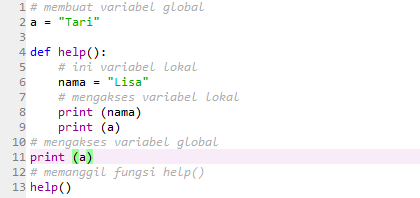
\includegraphics[width=10cm]{figures/variabel_global.PNG}
        \caption{Variabel Global}
    \end{figure}
    \item Variabel Lokal
    variabel lokal hanya bisa diakses dari dalam fungsi di mana ia di definisikan. Jika ada variabel yang dideklarasikan didalam suatu fungsi, variabel ini tidak ada kaitannya dengan variabel lain dengan nama yang sama diluar fungsi, dengan kata lain nama varabel hanya lokal untuk fungsi. 
    \begin{figure}[!htbp]
        \centering
        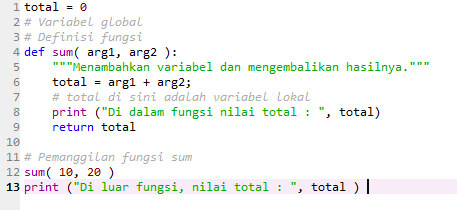
\includegraphics[width=10cm]{figures/variabel.PNG}
        \caption{Variabel Lokal}
        \label{}
    \end{figure}
\end{enumerate}
\newpage
\subsection{Tipe data}
    \begin{figure}[!htbp]
        \centering
        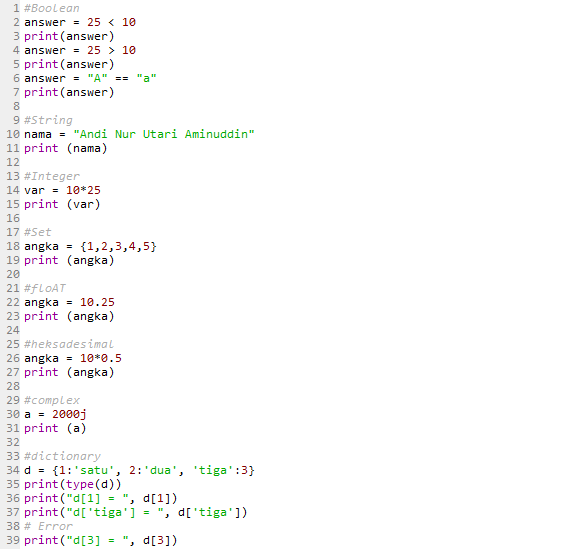
\includegraphics[width=15cm]{figures/tipedata.PNG}
    \end{figure}
        \begin{figure}[!htbp]
        \centering
        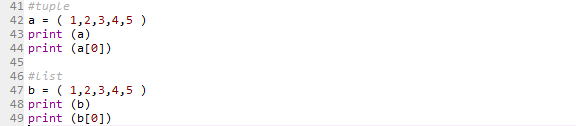
\includegraphics[width=15cm]{figures/tipedata2.PNG}
        \caption{Tipe data}
    \end{figure}
\newpage
\section{Bagaimana kode untuk meminta input dari user dan output ke layar}
    \begin{figure}[!htbp]
        \centering
        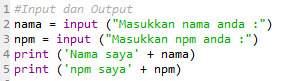
\includegraphics[width=8cm]{figures/inputdanoutput.PNG}
        \caption{Input dan Output}
        \label{}
    \end{figure}
\section{Operator dasar aritmatika dan bagaimana
mengubah string ke integer dan integer ke string}
\subsection{Operator dasar aritmatika}
\begin{enumerate}
    \item Pengurangan, operator ini digunakan untuk melakukan operasi perngurangan
        \begin{figure}[!htbp]
        \centering
        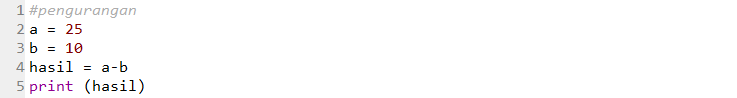
\includegraphics[width=15cm]{figures/pengurangan.PNG}
        \caption{Pengurangan}
        \label{}
    \end{figure}
    \item Pertambahanm, operator ini digunakan untuk melakukan operasi pertambahan
        \begin{figure}[!htbp]
        \centering
        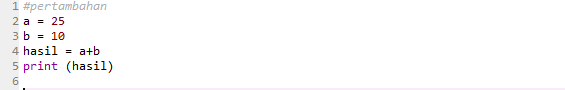
\includegraphics[width=15cm]{figures/tambah.PNG}
        \caption{Pertambahan}
        \label{}
    \end{figure}
    \newpage
    \item Perkalian, operator ini digunakan untuk melakukan operasi perkalian
        \begin{figure}[!htbp]
        \centering
        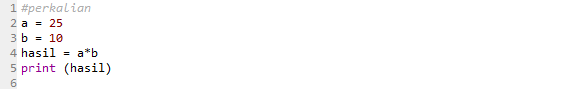
\includegraphics[width=15cm]{figures/kali.PNG}
        \caption{Perkalian}
        \label{}
    \end{figure}
    \item Pembagian, operator ini digunakan untuk melakukan operasi pembagian
        \begin{figure}[!htbp]
        \centering
        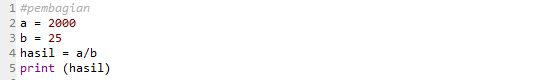
\includegraphics[width=15cm]{figures/bagi.PNG}
        \caption{Pembagian}
        \label{}
    \end{figure}
        \item Modulus, operator ini digunakan untuk melakukan operasi modulus
        \begin{figure}[!htbp]
        \centering
        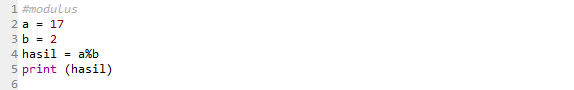
\includegraphics[width=15cm]{figures/modulus.PNG}
        \caption{Modulus}
        \label{}
    \end{figure}
    \item Perpangkatan, operator ini digunakan untuk melakukan operasi perpangkatan
        \begin{figure}[!htbp]
        \centering
        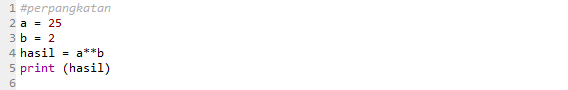
\includegraphics[width=15cm]{figures/pangkat.PNG}
        \caption{Perpangkatan}
        \label{}
    \end{figure}
    \newpage
        \item Pembulatan, operator ini digunakan untuk melakukan operasi pembulatan pada hasil pembagian
        \begin{figure}[!htbp]
        \centering
        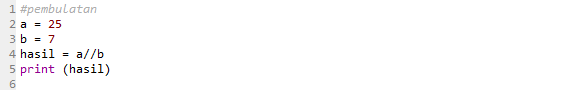
\includegraphics[width=15cm]{figures/pembulatan.PNG}
        \caption{Pembulatan}
        \label{}
    \end{figure}
\end{enumerate}
\subsection{Mengubah tipe data}
\begin{enumerate}
    \item Mengubah string ke integer
        \begin{figure}[!htbp]
        \centering
        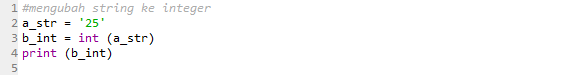
\includegraphics[width=15cm]{figures/str_int.PNG}
        \caption{Kode mengubah tipe data string ke integer}
    \end{figure}
        \item Mengubah integer ke string
        \begin{figure}[!htbp]
        \centering
        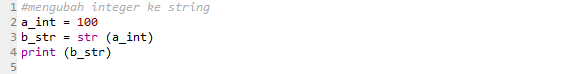
\includegraphics[width=15cm]{figures/int_str.PNG}
        \caption{Kode mengubah tipe data integer ke string}
    \end{figure}
\end{enumerate}
\section{Jenis-Jenis Perulangan}
\begin{enumerate}
    \item While Looping
     \begin{figure}[!htbp]
        \centering
        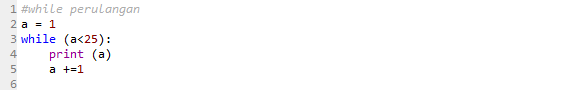
\includegraphics[width=15cm]{figures/while.PNG}
        \caption{Kode perulangan while}
    \end{figure}
    \newpage
    \item for Looping
        \begin{figure}[!htbp]
        \centering
        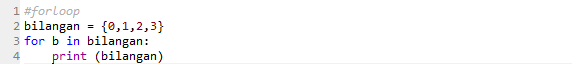
\includegraphics[width=15cm]{figures/for.PNG}
        \caption{Kode perulangan for}
    \end{figure}
    \item Nested Looping
     \begin{figure}[!htbp]
        \centering
        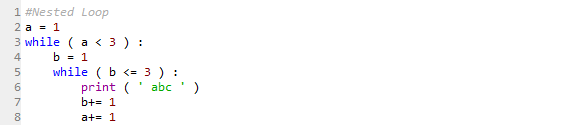
\includegraphics[width=15cm]{figures/nested.PNG}
        \caption{Kode perulangan nested}
    \end{figure}
\end{enumerate}
\section{Jenis-jenis kondisi}
\begin{enumerate}
    \item Kondisi IF
        \begin{figure}[!htbp]
        \centering
        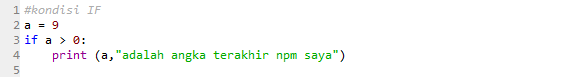
\includegraphics[width=15cm]{figures/if.PNG}
        \caption{Kode kondisi if}
    \end{figure}
    \item Kondisi Ifelse
        \begin{figure}[!htbp]
        \centering
        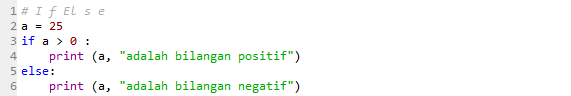
\includegraphics[width=15cm]{figures/ifelse.PNG}
        \caption{Kode Kondisi Ifelse}
    \end{figure}
    \newpage
    \item Kondisi Elif
        \begin{figure}[!htbp]
        \centering
        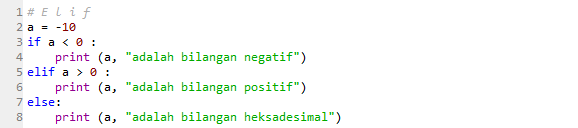
\includegraphics[width=15cm]{figures/elif.PNG}
        \caption{Kode Kondisi Elif}
    \end{figure}
    \item Kondisi dalam Kondisi
        \begin{figure}[!htbp]
        \centering
        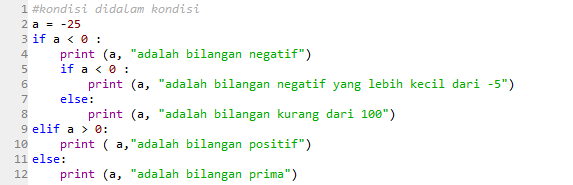
\includegraphics[width=15cm]{figures/kondisidalamkondisi.PNG}
        \caption{Kode Kondisi dalam Kondisi}
    \end{figure}
\end{enumerate}
\newpage
\section{Jenis-jenis error yang ditemukan dalam mengerjakan tugas ini}
\begin{enumerate}
    \item Syntax Error
    Syntax error adalah suatu keadaan atau kondisi ketika ada kesalahan penulisan kode pada program python hal ini menyebabkan program tidak dapat dijalankan. contohnya kesalahan pemberian titik dua atau tanda kutip. Output pemberitahuan error nya yaitu invalid syntax. Yang harus dilakukan saat terjadi syntax error pada kode program yaitu memperbaiki penulisan kodenya.
    \item Name Error
    Name error, yaitu exception yang muncul ketika melakukan eksekusi pada suatu program terhadapa lokal name dan global name tidak terdefinisi. error ini terjadi saat pemanggilan variabel yang tidak di definisikan atau memnaggil sebuah function yang tidak ada. Output pemberitahuan error nya yaitu name 'a' is not defined. Untuk mengatasi terjadi name error yaitu dengan memastikan variabel dan function yang akan dipanggil benar-benar ada dalam kode program dan tidak terjadi kesalahan penulisan.
    \item Type Error
    Type Error, yaitu suatu keadaan yang terjadi ketika melakukan eksekusi pada suatu operasi atau fungsi yang tipe datanya berbeda atau tidak sesuai dengan operasi yang akan dilakukan. Contoh kasusnya pada kesalahan tipe data antara string dan integer, kesalahan dalam input list,tupl dan dictionary. Cara penanganannya yaitu dengan mengkorversi variabel yang digunakan sesuai dengan tipe datanya.
    \item Identation error
    Identation error, yaitu tulisasn kode program yang menjorok. identation error akan terjadi ketika mengetik kode program namun tidak memperhatikan identasinya. Jika terjadi identasi maka program akan error. cara mengatasinya yaitu memperhatikan identasi saat menuliskan suatu program.
\end{enumerate}
\newpage
\section{Cara memakai Try Except}
    Salah satu bentuk penanganan error pada program python yaitu dengan menggunakan statement Try Except 
    \begin{figure}[!htbp]
        \centering
        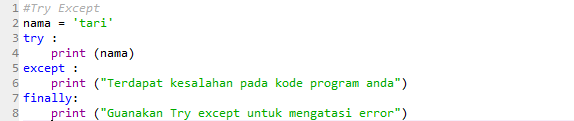
\includegraphics[width=15cm]{figures/tryexcept.PNG}
        \caption{Cara menggunakan Try Except}
    \end{figure}

    
    



    

    
    
 
